\documentclass[11pt,a4paper]{article}

% ==============================================================================
% CORE PACKAGES & GEOMETRY
% ==============================================================================
\usepackage[margin=1in,headheight=14pt]{geometry}
\usepackage[utf8]{inputenc}
\usepackage[T1]{fontenc}
\usepackage{amsmath,amssymb,amsfonts}
\usepackage{booktabs,tabularx,multirow,array}
\usepackage{graphicx}
\usepackage{xcolor}
\usepackage{enumitem}
\usepackage{caption}
\usepackage{subcaption}
\usepackage{fancyhdr}
\usepackage{titlesec}
\usepackage{listings}
\usepackage{tikz}
\usetikzlibrary{arrows.meta,positioning,shapes.geometric,backgrounds,fit,calc,trees}

% Set graphic paths to find training artifact images automatically
\graphicspath{
    {../models/checkpoints/civicpulse_v2_yolo11m/}
    {../models/checkpoints/civicpulse_v1_5class/}
    {models/checkpoints/civicpulse_v2_yolo11m/}
    {models/checkpoints/civicpulse_v1_5class/}
}

% ==============================================================================
% COLOR DEFINITIONS & HYPERLINK SETUP
% ==============================================================================
\definecolor{civicblue}{RGB}{14,75,140}
\definecolor{civicdark}{RGB}{20,30,45}
\definecolor{civicgray}{RGB}{90,100,115}
\definecolor{accentgreen}{RGB}{16,130,70}
\definecolor{accentred}{RGB}{180,40,40}
\definecolor{codebg}{RGB}{246,248,250}
\definecolor{bordergray}{RGB}{210,215,222}

\usepackage[
    colorlinks=true,
    linkcolor=civicblue,
    citecolor=civicblue,
    urlcolor=civicblue,
    filecolor=civicblue,
    pdfauthor={CivicPulse Engineering Team},
    pdftitle={CivicPulse: AI/ML Technical Documentation},
    pdfsubject={AI-Assisted Monsoon Civic Risk Intelligence & Response System},
    pdfkeywords={Computer Vision, YOLO11, ByteTrack, MiDaS, Depth Estimation, PostGIS, Drone Surveillance, Smart Cities}
]{hyperref}

% ==============================================================================
% TYPOGRAPHY & HEADINGS FORMATTING
% ==============================================================================
\titleformat{\section}
  {\normalfont\Large\bfseries\color{civicdark}}{\thesection}{1em}{}[\titlerule]
\titleformat{\subsection}
  {\normalfont\large\bfseries\color{civicdark}}{\thesubsection}{1em}{}
\titleformat{\subsubsection}
  {\normalfont\normalsize\bfseries\color{civicdark}}{\thesubsubsection}{1em}{}

\setlength{\parskip}{0.5em}
\setlength{\parindent}{0pt}

% Header and Footer
\pagestyle{fancy}
\fancyhf{}
\fancyhead[L]{\small\color{civicgray}\textbf{CivicPulse} \textbar\ AI/ML Technical Documentation}
\fancyhead[R]{\small\color{civicgray}ELCIA Smart City Challenge 2026}
\fancyfoot[L]{\small\color{civicgray}Engineering Technical Report --- CivicPulse Subsystem}
\fancyfoot[R]{\small\color{civicgray}Page \thepage}
\renewcommand{\headrulewidth}{0.4pt}
\renewcommand{\footrulewidth}{0.4pt}

% Code listing configuration
\lstset{
    backgroundcolor=\color{codebg},
    basicstyle=\small\ttfamily,
    breaklines=true,
    frame=single,
    rulecolor=\color{bordergray},
    keywordstyle=\color{civicblue}\bfseries,
    commentstyle=\color{civicgray}\itshape,
    stringstyle=\color{accentgreen},
    showstringspaces=false,
    tabsize=2
}

% ==============================================================================
% DOCUMENT BEGIN
% ==============================================================================
\begin{document}

% ------------------------------------------------------------------------------
% TITLE BLOCK
% ------------------------------------------------------------------------------
\begin{titlepage}
    \centering
    \vspace*{1.5cm}
    
    {\Huge\bfseries\color{civicdark} CivicPulse}\\[0.4cm]
    {\LARGE\bfseries\color{civicblue} AI/ML Technical Documentation}\\[0.3cm]
    {\large\textit{AI-Assisted Monsoon Civic Risk Intelligence \& Response System}}\\[1.2cm]
    
    \rule{\textwidth}{1.2pt}\\[0.6cm]
    
    \textbf{Challenge Track:} ELCIA Smart City Drone-AI Challenge 2026\\
    \textbf{Domain Focus:} Monsoon Resilience \textbullet\ Road Networks \textbullet\ Civic Infrastructure\\
    \textbf{Target Deployment:} Electronics City Industrial Township Authority (ELCIA), Bengaluru\\[0.8cm]
    
    \rule{\textwidth}{1.2pt}\\[1.5cm]
    
    \begin{minipage}{0.48\textwidth}
        \begin{flushleft} \large
            \textbf{Evaluated Subcomponents:}\\
            YOLO11m-seg Instance Segmentation\\
            Custom ByteTrack Temporal Association\\
            MiDaS DPT-Large Relative Depth\\
            PostgreSQL / PostGIS Spatial Storage\\
            FastAPI \& React Operations Stack
        \end{flushleft}
    \end{minipage}
    \begin{minipage}{0.48\textwidth}
        \begin{flushright} \large
            \textbf{Document Classification:}\\
            Technical Engineering Report\\
            Version: 2.3.0 (Evidence-Grounded Head)\\
            Date: September 2026\\
            Status: Implemented \& Experimentally Evaluated
        \end{flushright}
    \end{minipage}
    
    \vfill
    {\small\color{civicgray} Electronics City Industrial Association (ELCIA) \textbullet\ Bengaluru, Karnataka, India}
\end{titlepage}

\pagenumbering{roman}
\tableofcontents
\newpage
\pagenumbering{arabic}
\setcounter{page}{1}

% ==============================================================================
% 1. ABSTRACT
% ==============================================================================
\section{Abstract}
Civic infrastructure in urban industrial townships experiences rapid surface degradation during severe monsoon seasons. Traditional ground-level reporting suffers from observational latency, incomplete spatial coverage, and inconsistent manual triage. \textbf{CivicPulse} introduces an automated, multi-stage aerial computer vision and geospatial intelligence pipeline designed for stream-based and offline monsoon hazard triage. Operating on aerial drone surveillance video accompanied by synchronized DJI GPS/SRT telemetry subtitles, CivicPulse executes a multi-stage machine learning pipeline consisting of: (1) multi-class instance segmentation via a fine-tuned \textbf{YOLO11m-seg} network; (2) multi-frame object tracking and identity preservation via an optimized \textbf{ByteTrack} formulation; (3) temporal persistence filtering and optical Laplacian surface-smoothness verification gates; (4) selective zero-shot relative inverse disparity estimation using \textbf{MiDaS / DPT-Large}; (5) explainable multi-factor civic severity scoring ($0.0$--$10.0$) and operational priority mapping ($\text{P1}$/$\text{P2}$/$\text{P3}$); and (6) timestamp-based GPS coordinate matching with automated \textbf{PostgreSQL / PostGIS} persistence, exposed via a \textbf{FastAPI} backend to a \textbf{React} operations dashboard. This document provides a code-grounded, evidence-first technical exposition of the algorithms, architectural decisions, model evolution, measured validation metrics, hardware profiles, and operational safeguards governing the CivicPulse AI/ML subsystem.

% ==============================================================================
% 2. SYSTEM OVERVIEW
% ==============================================================================
\section{System Overview}
The CivicPulse AI/ML subsystem transforms moving-camera aerial video streams into verified, geolocated, and deduplicated civic hazard records. In industrial townships such as Electronics City (ELCIA), monsoons trigger infrastructure failures including hazardous road waterlogging, structural potholes, drainage culvert overflows, damaged walkways, and uncovered manholes. 

\begin{figure}[htbp]
\centering
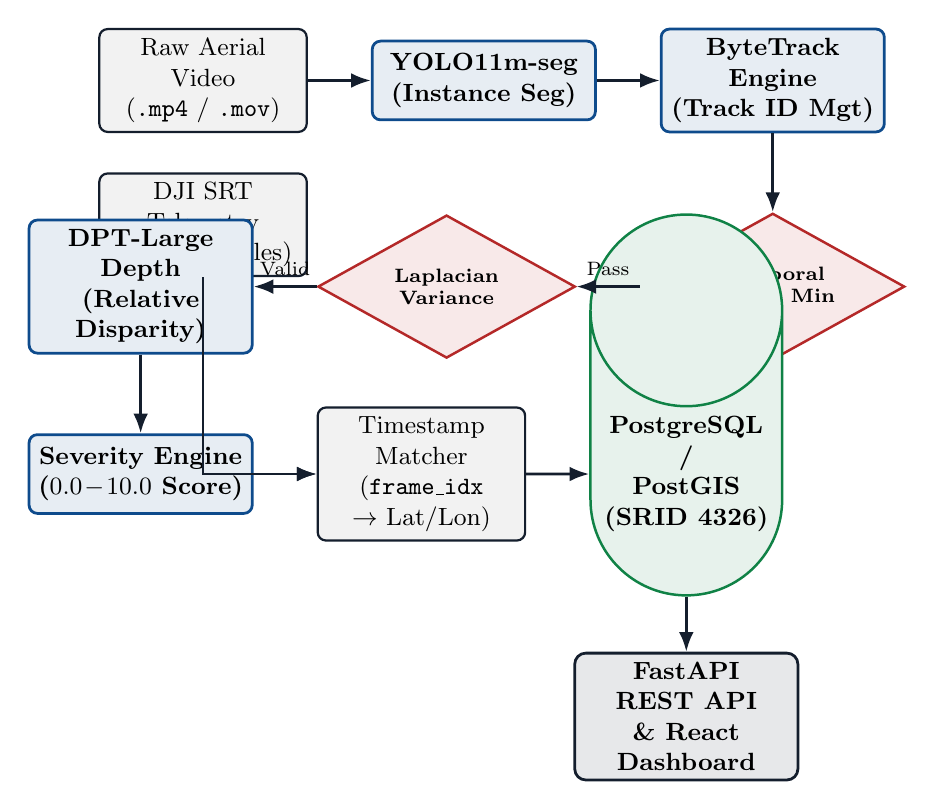
\begin{tikzpicture}[
    node distance=0.85cm and 0.6cm,
    every node/.style={font=\small, align=center},
    inputbox/.style={rectangle, rounded corners=3pt, draw=civicdark, fill=gray!10, text width=2.4cm, minimum height=1.0cm, line width=0.8pt},
    mlbox/.style={rectangle, rounded corners=3pt, draw=civicblue, fill=civicblue!10, text width=2.6cm, minimum height=1.0cm, line width=1.0pt, font=\small\bfseries},
    gatebox/.style={diamond, draw=accentred, fill=accentred!10, text width=1.8cm, minimum height=1.0cm, line width=0.9pt, aspect=1.8, font=\scriptsize\bfseries},
    dbbox/.style={cylinder, shape border rotate=90, draw=accentgreen, fill=accentgreen!10, text width=2.2cm, minimum height=1.1cm, line width=0.9pt, font=\small\bfseries},
    uibox/.style={rectangle, rounded corners=4pt, draw=civicdark, fill=civicdark!10, text width=2.6cm, minimum height=1.0cm, line width=1.0pt, font=\small\bfseries},
    arr/.style={-{Latex[length=2.5mm]}, line width=1.0pt, draw=civicdark}
]

% Row 1: Inputs & ML
\node[inputbox] (video) {Raw Aerial Video\\(\texttt{.mp4} / \texttt{.mov})};
\node[inputbox, below=0.5cm of video] (srt) {DJI SRT Telemetry\\(GPS Subtitles)};
\node[mlbox, right=0.8cm of video] (yolo) {YOLO11m-seg\\(Instance Seg)};
\node[mlbox, right=0.8cm of yolo] (bytetrack) {ByteTrack Engine\\(Track ID Mgt)};

% Row 2: Validation Gates & Secondary ML
\node[gatebox, below=1.0cm of bytetrack] (temporal) {Temporal\\Hits $\ge$ Min};
\node[gatebox, left=0.8cm of temporal] (texture) {Laplacian\\Variance};
\node[mlbox, left=0.8cm of texture] (depth) {DPT-Large Depth\\(Relative Disparity)};

% Row 3: Severity & Backend
\node[mlbox, below=1.0cm of depth] (severity) {Severity Engine\\($0.0 - 10.0$ Score)};
\node[inputbox, right=0.8cm of severity] (sync) {Timestamp Matcher\\(\texttt{frame\_idx} $\to$ Lat/Lon)};
\node[dbbox, right=0.8cm of sync] (postgis) {PostgreSQL /\\PostGIS (SRID 4326)};
\node[uibox, below=0.7cm of postgis] (dashboard) {FastAPI REST API\\\& React Dashboard};

% Connections
\draw[arr] (video) -- (yolo);
\draw[arr] (yolo) -- (bytetrack);
\draw[arr] (bytetrack) -- (temporal);
\draw[arr] (temporal) -- node[above, font=\scriptsize] {Pass} (texture);
\draw[arr] (texture) -- node[above, font=\scriptsize] {Valid} (depth);
\draw[arr] (depth) -- (severity);
\draw[arr] (srt) |- (sync);
\draw[arr] (severity) -- (sync);
\draw[arr] (sync) -- (postgis);
\draw[arr] (postgis) -- (dashboard);

\end{tikzpicture}
\caption{End-to-end CivicPulse AI/ML pipeline architecture and backend integration flow.}
\label{fig:e2e_architecture}
\end{figure}

The pipeline enforces several engineering design principles:
\begin{enumerate}[leftmargin=*]
    \item \textbf{Polygonal Mask Segmentation:} Extracting pixel-accurate segmentation masks rather than coarse bounding boxes to measure actual hazard surface coverage.
    \item \textbf{Track Deduplication (1 Physical Hazard = 1 Incident):} Associating repeated bounding boxes across consecutive frames using ByteTrack Kalman filtering to prevent duplicate records.
    \item \textbf{Timestamp-Based GPS Geolocation:} Associating video frame timestamps ($t = i / \text{FPS}$) with parsed subtitle flight logs to attach geospatial coordinates.
    \item \textbf{Spatial Integrity \& Decoupled Zones:} Ensuring that incidents detected outside predefined administrative operational zones retain exact raw GPS coordinates without artificial fallback to default sectors.
\end{enumerate}

% ==============================================================================
% 3. END-TO-END AI/ML ARCHITECTURE
% ==============================================================================
\section{End-to-End AI/ML Architecture}
The CivicPulse machine learning subsystem executes as an asynchronous, decoupled pipeline implemented in \texttt{src/detection/video\_tracker.py} and invoked via the CLI runner \texttt{src/detection/runner.py} or the job management service \texttt{src/services/processing\_job\_manager.py}.

The processing pipeline executes across sequential stages:
\begin{enumerate}[leftmargin=*]
    \item \textbf{Ingestion \& Video Demuxing:} The input video container is parsed using OpenCV \texttt{cv2.VideoCapture}, reading native resolution $(W, H)$, frame rate ($\text{FPS}$), and total frame count.
    \item \textbf{Deep Feature Extraction \& Segmentation:} Each frame $F_t$ is normalized and processed by \textbf{YOLO11m-seg} at inference resolution ($640\times 640$ pixels).
    \item \textbf{Track State Association:} Detections are routed through a parameterized \textbf{ByteTrack} tracker to match bounding boxes and spatial masks across temporal horizons.
    \item \textbf{Multi-Stage Validation Gating:} Candidate tracks are filtered by a temporal hit counter ($\ge N$ consecutive hits) and Laplacian texture variance analysis.
    \item \textbf{Monocular Relative Depth Profiling:} For structural cavity hazards (\texttt{pothole}), bounding box regions are processed by \textbf{DPT-Large} to extract relative depth and disparity features.
    \item \textbf{Severity Synthesis:} Multi-factor scoring combines mask surface ratio, depth disparity, detection confidence, and roadway criticality into a normalized score $\in [0.0, 10.0]$ and maps to priority tiers ($\text{P1}, \text{P2}, \text{P3}$).
    \item \textbf{Geospatial Synchronization \& Artifact Export:} Frame index $t$ is mapped to parsed DJI GPS telemetry via second-level timestamp matching, exporting cropped evidence JPEGs, an H.264 browser-compatible annotated MP4 video, and a structured \texttt{hazard\_telemetry.json} manifest.
    \item \textbf{Database Ingestion:} The backend service (\texttt{src/services/ml\_ingestion\_service.py}) parses the telemetry manifest, inserting relational and PostGIS spatial entities.
\end{enumerate}

% ==============================================================================
% 4. INPUT DATA
% ==============================================================================
\section{Input Data}

\subsection{Drone Video Stream}
CivicPulse processes aerial video recorded with standard UAV camera sensors. Compatible and evaluated input characteristics are summarized in Table~\ref{tab:input_data_spec}.

\begin{table}[htbp]
\centering
\small
\caption{Observed, configured, and compatible input data characteristics in CivicPulse.}
\label{tab:input_data_spec}
\begin{tabularx}{\textwidth}{l l X}
\toprule
\textbf{Parameter} & \textbf{Observed / Configured / Compatible} & \textbf{Engineering Significance} \\
\midrule
Container Formats & \texttt{.mp4} (Observed), \texttt{.mov} (Compatible) & Decoded via OpenCV \texttt{cv2.VideoCapture}; H.264/H.265 streams supported. \\
Spatial Resolution & $1920\times 1080$ FHD (Observed), Arbitrary (Compatible) & Evaluated on 1080p demo flight; resized dynamically to $640\times 640$ during inference. \\
Temporal Frame Rate & 30 FPS (Observed), 24 / 29.97 / 60 FPS (Compatible) & Read dynamically via OpenCV \texttt{CAP\_PROP\_FPS}; computes elapsed time $t = i / \text{FPS}$. \\
Camera Vantage & Nadir to Oblique ($45^\circ$--$90^\circ$) (Observed) & Tested on aerial UAV footage; oblique angles enable relative depth disparity profiling. \\
Telemetry Format & DJI Sidecar Subtitles (\texttt{.srt}) (Observed) & Parsed via regex in \texttt{gps\_parser.py} for millisecond/second-level GPS tags. \\
\bottomrule
\end{tabularx}
\end{table}

\subsection{GPS / SRT Telemetry}
DJI drone platforms generate synchronized subtitle sidecar files (\texttt{.srt}) containing periodic telemetry records. CivicPulse implements a dedicated regex-based subtitle parser in \texttt{scripts/gps\_parser.py} capable of ingesting both modern bracketed DJI formats and legacy string formats:
\begin{itemize}[leftmargin=*]
    \item \textbf{Modern Bracket Syntax:} \texttt{[latitude: 12.845012] [longitude: 77.663845] [altitude: 45.2]}
    \item \textbf{Legacy Syntax:} \texttt{GPS (12.845012, 77.663845, 45.2M)}
\end{itemize}

\subsection{Video--Telemetry Timestamp Association}
Video frames and subtitle timestamps are aligned using direct timestamp matching. For frame index $i$ sampled at frame rate $\text{FPS}$, the elapsed video timestamp in seconds is:
\begin{equation}
t_{\text{sec}} = \frac{i}{\text{FPS}}
\end{equation}
The integer second timestamp is formatted as $\text{HH:MM:SS}$ and matched against parsed time blocks from the SRT telemetry stream. If an exact match is unavailable, the parser associates the nearest preceding timestamp or falls back to the final recorded flight coordinate. Coordinate interpolation is not performed; raw recorded telemetry coordinates are preserved. If telemetry is absent, coordinates default to \texttt{None}, flagging the flight for manual operator coordinate verification.

% ==============================================================================
% 5. OBJECT DETECTION --- YOLOV11M SEGMENTATION
% ==============================================================================
\section{Object Detection --- YOLOv11m Segmentation}

\subsection{Architectural Justification}
Standard bounding-box object detectors fail in municipal waterlogging and drainage monitoring because civic hazards follow non-rectangular, fractal, and irregular geometries. CivicPulse deploys \textbf{YOLO11m-seg}, the medium-scale instance segmentation variant of the Ultralytics YOLO11 architecture, incorporating C3k2 cross-stage partial blocks, SPPF (Spatial Pyramid Pooling - Fast), and C2PSA (Cross-Stage Partial with Pointwise Spatial Attention) mechanisms.

\subsection{Hazard Class Taxonomy \& Parameters}
CivicPulse operates on a 5-class hazard taxonomy defined in \texttt{configs/config.yaml} and enforced across the codebase via \texttt{src/core/classes.py}. Table~\ref{tab:class_taxonomy} details the configuration parameters.

\begin{table}[htbp]
\centering
\small
\caption{CivicPulse 5-class hazard taxonomy, detection floors, and validation parameters.}
\label{tab:class_taxonomy}
\begin{tabularx}{\textwidth}{c l c c c c c X}
\toprule
\textbf{ID} & \textbf{Class Name} & \textbf{Conf} & \textbf{Color (BGR)} & \textbf{Min Hits} & \textbf{Depth?} & \textbf{Smooth?} & \textbf{Severity Mult.} \\
\midrule
0 & \texttt{damaged\_footpath} & 0.15 & $(0, 255, 0)$ & 2 & False & False & $1.0\times$ \\
1 & \texttt{drainage\_overflow} & 0.30 & $(0, 255, 255)$ & 2 & False & False & $1.0\times$ \\
2 & \texttt{open\_manhole} & 0.60 & $(200, 0, 200)$ & 3 & False & False & $1.3\times$ (High Risk) \\
3 & \texttt{pothole} & 0.30 & $(40, 50, 230)$ & 2 & True & False & $1.1\times$ \\
4 & \texttt{waterlogging} & 0.30 & $(235, 150, 50)$ & 5 & False & True & $1.0\times$ \\
\bottomrule
\end{tabularx}
\end{table}

\subsection{Inference Pipeline \& Polygon Extraction}
For each video frame $F_t \in \mathbb{R}^{H \times W \times 3}$, inference proceeds through \texttt{YOLOSegmentor.track\_frame()}:
\begin{enumerate}[leftmargin=*]
    \item \textbf{Input Scaling:} The frame is resized to $640\times 640$ with aspect-ratio letterbox padding.
    \item \textbf{Forward Pass:} The model generates bounding boxes $B_k = [x_1, y_1, x_2, y_2]$, confidence scores $c_k \in [0, 1]$, class predictions $y_k \in \{0,\dots,4\}$, and prototype mask coefficients.
    \item \textbf{Mask Decoding:} Raw mask coefficients are multiplied by prototype masks and thresholded at $0.5$, yielding binary mask $M_k \in \{0, 1\}^{H \times W}$.
    \item \textbf{Contour Extraction:} Binary masks are converted to integer boundary polygons $P_k = \{(x_j, y_j)\}_{j=1}^m$ using \texttt{cv2.findContours}.
    \item \textbf{Geometric Filtering:} Polygons with surface area $A_k = \text{cv2.contourArea}(P_k) < 50.0\text{ pixels}$ are rejected as noise artifacts.
    \item \textbf{Centroid Calculation:} Spatial centroids $(C_x, C_y)$ are computed using image spatial moments:
    \begin{equation}
    C_x = \frac{M_{10}}{M_{00}}, \quad C_y = \frac{M_{01}}{M_{00}}, \quad \text{where } M_{pq} = \sum_{x,y} x^p y^q M_k(x, y)
    \end{equation}
\end{enumerate}

\subsection{Execution Hardware Resolution}
The segmentation engine dynamically selects compute backends:
\begin{equation}
\text{Device} = \begin{cases}
\texttt{cuda}, & \text{if } \texttt{torch.cuda.is\_available()} \\
\texttt{mps}, & \text{if } \texttt{torch.backends.mps.is\_available()} \text{ (Apple Silicon)} \\
\texttt{cpu}, & \text{otherwise (Fallback)}
\end{cases}
\end{equation}

% ==============================================================================
% 6. OBJECT TRACKING --- BYTETRACK
% ==============================================================================
\section{Object Tracking --- ByteTrack}

\subsection{The Multi-Frame Association Problem}
When a drone cruises over a roadway at $5\text{ m/s}$, a single $2\text{ m}$ pothole remains visible across $60$--$120$ successive video frames. Without temporal tracking, an object detector registers $120$ distinct detection records, duplicating database records and triggering redundant field dispatch notifications.

\subsection{ByteTrack Parameterization in CivicPulse}
CivicPulse integrates an optimized \textbf{ByteTrack} tracker configured via \texttt{configs/custom\_bytetrack.yaml}. ByteTrack performs temporal association of detections across successive frames without requiring an appearance-based Re-ID feature extractor.

\begin{figure}[htbp]
\centering
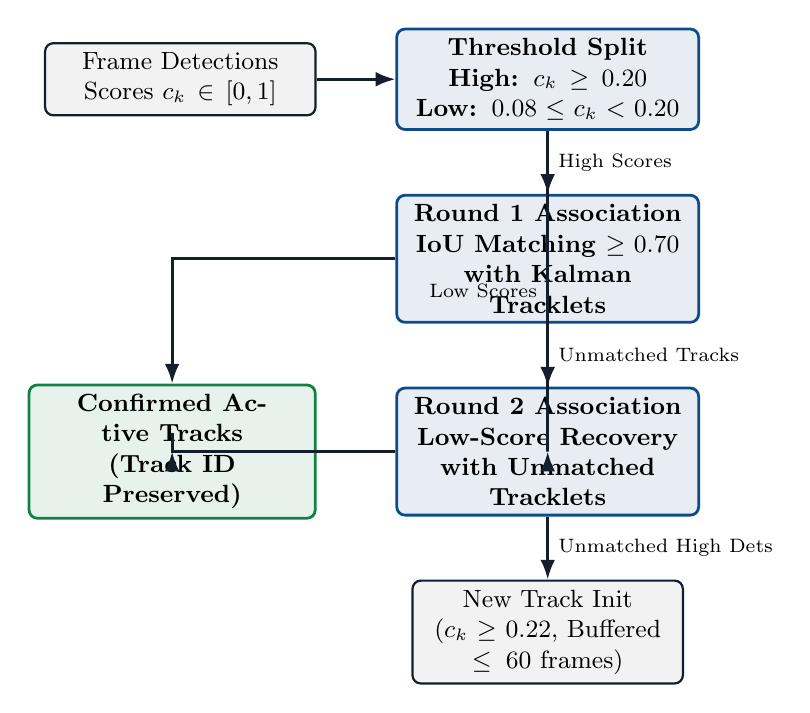
\begin{tikzpicture}[
    node distance=0.7cm and 0.7cm,
    every node/.style={font=\small, align=center},
    stagebox/.style={rectangle, rounded corners=3pt, draw=civicdark, fill=gray!10, text width=3.2cm, minimum height=0.9cm, line width=0.8pt},
    matchbox/.style={rectangle, rounded corners=3pt, draw=civicblue, fill=civicblue!10, text width=3.6cm, minimum height=0.9cm, line width=1.0pt, font=\small\bfseries},
    trackbox/.style={rectangle, rounded corners=3pt, draw=accentgreen, fill=accentgreen!10, text width=3.4cm, minimum height=0.9cm, line width=1.0pt, font=\small\bfseries},
    arr/.style={-{Latex[length=2.5mm]}, line width=1.0pt, draw=civicdark}
]

\node[stagebox] (detections) {Frame Detections\\Scores $c_k \in [0, 1]$};
\node[matchbox, right=1.0cm of detections] (split) {Threshold Split\\High: $c_k \ge 0.20$\\Low: $0.08 \le c_k < 0.20$};
\node[matchbox, below=0.8cm of split] (first_match) {Round 1 Association\\IoU Matching $\ge 0.70$\\with Kalman Tracklets};
\node[matchbox, below=0.8cm of first_match] (second_match) {Round 2 Association\\Low-Score Recovery\\with Unmatched Tracklets};
\node[trackbox, left=1.0cm of second_match] (active_tracks) {Confirmed Active Tracks\\(Track ID Preserved)};
\node[stagebox, below=0.8cm of second_match] (new_tracks) {New Track Init\\($c_k \ge 0.22$, Buffered $\le 60\text{ frames}$)};

\draw[arr] (detections) -- (split);
\draw[arr] (split) -- node[right, font=\scriptsize] {High Scores} (first_match);
\draw[arr] (first_match) -- node[right, font=\scriptsize] {Unmatched Tracks} (second_match);
\draw[arr] (split) |- node[near start, left, font=\scriptsize] {Low Scores} (second_match);
\draw[arr] (first_match) -| (active_tracks);
\draw[arr] (second_match) -| (active_tracks);
\draw[arr] (second_match) -- node[right, font=\scriptsize] {Unmatched High Dets} (new_tracks);

\end{tikzpicture}
\caption{Two-stage ByteTrack association pipeline utilized for hazard track preservation.}
\label{fig:bytetrack_flow}
\end{figure}

The tracking hyperparameters in \texttt{configs/custom\_bytetrack.yaml} are configured as follows:
\begin{itemize}[leftmargin=*]
    \item \texttt{track\_high\_thresh: 0.20}: High-confidence threshold for initial Kalman association.
    \item \texttt{track\_low\_thresh: 0.08}: Low-confidence threshold allowing recovery of partially occluded or blurred defects during camera motion.
    \item \texttt{new\_track\_thresh: 0.22}: Minimum score required to initialize a new track ID.
    \item \texttt{track\_buffer: 60}: Frame retention buffer ($2.0\text{ seconds}$ at $30\text{ FPS}$) maintaining lost tracks across transient occlusions.
    \item \texttt{match\_thresh: 0.70}: Intersection-over-Union (IoU) spatial matching threshold.
    \item \texttt{fuse\_score: True}: Fuses detection probability with Kalman state uncertainty.
\end{itemize}

% ==============================================================================
% 7. TEMPORAL PERSISTENCE / HAZARD CONFIRMATION
% ==============================================================================
\section{Temporal Persistence / Hazard Confirmation}
To filter transient false positives caused by brief visual artifacts (e.g., sensor glint, moving shadow, camera shake), CivicPulse implements a dual-stage validation gate before promoting a tracked defect to a confirmed incident.

\subsection{Temporal Hit Counter Gate}
For every active track ID $\tau$, the pipeline maintains an accumulation counter $H(\tau)$. A track is promoted to confirmed status only when:
\begin{equation}
H(\tau) \ge \text{min\_hits}(y)
\end{equation}
where $\text{min\_hits}(y)$ is class-specific:
\begin{itemize}[leftmargin=*]
    \item \textbf{Waterlogging ($\text{min\_hits} = 5$):} Requires $5$ frames ($\approx 0.17\text{ s}$) of continuous observation to filter brief road reflections.
    \item \textbf{Open Manhole ($\text{min\_hits} = 3$):} Requires $3$ frames ($\approx 0.10\text{ s}$) to verify circular void geometry.
    \item \textbf{Pothole / Drainage / Footpath ($\text{min\_hits} = 2$):} Requires $2$ frames ($\approx 0.07\text{ s}$) of geometric consistency.
\end{itemize}

\subsection{Optical Surface Texture Gate}
Wet asphalt exhibits dark specular reflections that visual segmentors may confuse with standing water pools. For hazards where \texttt{requires\_smooth\_surface: true} (\texttt{waterlogging}), the pipeline extracts the bounding box region of interest (ROI) and computes the variance of the Laplacian:
\begin{equation}
\sigma_{\text{Laplacian}}^2 = \text{Var}\left(\nabla^2 I_{\text{gray}}\right)
\end{equation}
Empirical calibration demonstrates:
\begin{itemize}[leftmargin=*]
    \item \textbf{Dry / Textured Asphalt:} $\sigma_{\text{Laplacian}}^2 > 600.0$ (high granular aggregate texture).
    \item \textbf{Standing Water Body:} $\sigma_{\text{Laplacian}}^2 < 550.0$ (smooth optical mirror surface).
\end{itemize}
Candidate waterlogging detections with $\sigma_{\text{Laplacian}}^2 \ge 550.0$ are discarded.

\subsection{Tracking Lifecycle \& Duration Tracking}
For every verified track ID, CivicPulse records the initial observation timestamp $t_{\text{first}}$ and updates the terminal timestamp $t_{\text{last}}$ on every frame hit. Upon video completion, the observation duration is computed:
\begin{equation}
\Delta t = \max\left(0.0, t_{\text{last}} - t_{\text{first}}\right)
\end{equation}
This duration is persisted to the database column \texttt{incidents.duration\_seconds}.

% ==============================================================================
% 8. DEPTH ESTIMATION --- MIDAS / DPT
% ==============================================================================
\section{Depth Estimation --- MiDaS / DPT}

\subsection{Purpose and Scope}
While 2D instance segmentation determines hazard surface area, pothole severity is strongly influenced by cavity depth. CivicPulse integrates \textbf{MiDaS / DPT-Large} (Dense Prediction Transformer) via PyTorch Hub (\texttt{intel-isl/MiDaS}, \texttt{DPT\_Large}) to compute relative monocular inverse depth maps.

\subsection{Mathematical Model \& Relative Scaling}
Monocular vision networks without hardware LiDAR or calibrated stereo baselines cannot resolve absolute physical metric distance due to scale-depth ambiguity. DPT-Large outputs a relative inverse disparity map $d(x, y) \propto 1 / Z(x, y)$. 

In \texttt{DepthEstimator.estimate\_depth()}, the raw disparity prediction $D \in \mathbb{R}^{H \times W}$ is normalized to an 8-bit relative scale $[0, 255]$:
\begin{equation}
D_{\text{norm}}(x, y) = \begin{cases}
255 \times \frac{D(x, y) - \min(D)}{\max(D) - \min(D)}, & \text{if } \max(D) > \min(D) \\
0, & \text{otherwise}
\end{cases}
\end{equation}

\subsection{Relative Depth Drop Metric}
For structural potholes (\texttt{needs\_depth: true}), the pipeline masks the normalized depth map with the hazard polygon $P_k$:
\begin{equation}
\delta_{\text{rel}} = \frac{1}{|P_k|} \sum_{(x,y) \in P_k} \frac{D_{\text{norm}}(x, y)}{255.0} \in [0.0, 1.0]
\end{equation}
A higher value of $\delta_{\text{rel}}$ indicates local cavity depression relative to surrounding road plane pixels.

% ==============================================================================
% 9. SEVERITY / RISK ASSESSMENT
% ==============================================================================
\section{Severity / Risk Assessment}
CivicPulse deploys a hybrid, explainable risk formulation combining geometric polygon area ratio, depth disparity, detection certainty, and road criticality.

\subsection{Mathematical Formulation}
Let $A_{\text{poly}}$ be the hazard polygon pixel area, $A_{\text{frame}} = W \times H$ be the total frame area, and $R_{\text{cov}} = A_{\text{poly}} / A_{\text{frame}}$ be the raw coverage ratio. The normalized coverage metric is defined as:
\begin{equation}
\text{Cov}_{\text{norm}} = \min\left(1.0, R_{\text{cov}} \times 10.0\right)
\end{equation}

The severity score $S_{\text{raw}} \in [0.0, 10.0]$ is computed as:
\begin{equation}
S_{\text{raw}} = \left( w_{\text{cov}} \cdot \text{Cov}_{\text{norm}} + w_{\text{conf}} \cdot c_k + w_{\text{crit}} \cdot K_{\text{road}} \right) \times 10.0 \times M_{\text{class}}
\end{equation}
where:
\begin{itemize}[leftmargin=*]
    \item $w_{\text{cov}} = 0.45$: Weight assigned to spatial hazard footprint.
    \item $w_{\text{conf}} = 0.25$: Weight assigned to model detection confidence.
    \item $w_{\text{crit}} = 0.30$: Weight assigned to road infrastructure criticality index ($K_{\text{road}} \in [0.4, 1.0]$: Arterial $= 1.0$, Sector $= 0.8$, Alley $= 0.4$).
    \item $M_{\text{class}}$: Per-class risk multiplier (\texttt{open\_manhole}: $1.3\times$, \texttt{pothole}: $1.1\times$, others: $1.0\times$).
\end{itemize}

The final normalized severity score $S \in [1.0, 10.0]$ is clamped:
\begin{equation}
S = \text{round}\left(\min\left(10.0, \max\left(1.0, S_{\text{raw}}\right)\right), 1\right)
\end{equation}

\subsection{Operational Priority Assignment}
Severity scores map to operational triage categories:
\begin{equation}
\text{Priority} = \begin{cases}
\textbf{P1 (Critical):} & S \ge 6.5 \implies \text{Immediate Emergency Dispatch (Dewatering Pump / Manhole Barrier)} \\
\textbf{P2 (High):} & 4.0 \le S < 6.5 \implies \text{Scheduled 24-Hour Maintenance Queue} \\
\textbf{P3 (Routine):} & S < 4.0 \implies \text{Monitoring Queue (Erosion \& Silt Inspection)}
\end{cases}
\end{equation}

% ==============================================================================
% 10. TIMESTAMP-BASED GPS GEOLOCATION
% ==============================================================================
\section{Timestamp-Based GPS Geolocation}

\subsection{Coordinate Association Pipeline}
Figure~\ref{fig:gps_sync_flow} illustrates the transformation from video frame index to indexed PostGIS point.

\begin{figure}[htbp]
\centering
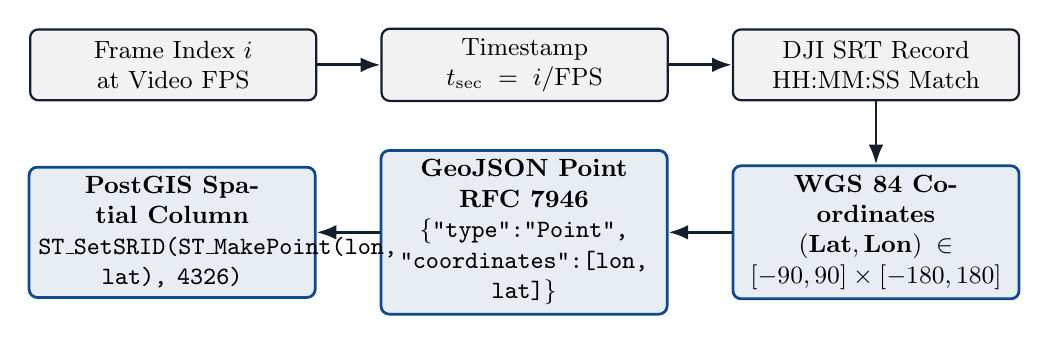
\begin{tikzpicture}[
    node distance=0.7cm and 0.8cm,
    every node/.style={font=\small, align=center},
    stepbox/.style={rectangle, rounded corners=3pt, draw=civicdark, fill=gray!10, text width=3.4cm, minimum height=0.9cm, line width=0.8pt},
    databox/.style={rectangle, rounded corners=3pt, draw=civicblue, fill=civicblue!10, text width=3.4cm, minimum height=0.9cm, line width=1.0pt, font=\small\bfseries},
    arr/.style={-{Latex[length=2.5mm]}, line width=1.0pt, draw=civicdark}
]

\node[stepbox] (fidx) {Frame Index $i$\\at Video FPS};
\node[stepbox, right=0.8cm of fidx] (tsec) {Timestamp\\$t_{\text{sec}} = i / \text{FPS}$};
\node[stepbox, right=0.8cm of tsec] (srt) {DJI SRT Record\\$\text{HH:MM:SS}$ Match};
\node[databox, below=0.8cm of srt] (wgs84) {WGS 84 Coordinates\\$(\text{Lat}, \text{Lon}) \in [-90, 90] \times [-180, 180]$};
\node[databox, left=0.8cm of wgs84] (geojson) {GeoJSON Point RFC 7946\\\texttt{\{"type":"Point", "coordinates":[lon, lat]\}}};
\node[databox, left=0.8cm of geojson] (postgis) {PostGIS Spatial Column\\\texttt{ST\_SetSRID(ST\_MakePoint(lon, lat), 4326)}};

\draw[arr] (fidx) -- (tsec);
\draw[arr] (tsec) -- (srt);
\draw[arr] (srt) -- (wgs84);
\draw[arr] (wgs84) -- (geojson);
\draw[arr] (geojson) -- (postgis);

\end{tikzpicture}
\caption{Timestamp-based video-to-GPS telemetry association and PostGIS spatial indexing flow.}
\label{fig:gps_sync_flow}
\end{figure}

\subsection{Distinction: Operational Zones vs. Incident Coordinates}
CivicPulse decouples administrative operational zones from exact incident coordinates:
\begin{itemize}[leftmargin=*]
    \item \textbf{Operational Zone (\texttt{zones} table):} Represents administrative macro-boundaries (e.g., \texttt{EC-01: Phase 1 West}, \texttt{EC-02: Phase 1 East}, \texttt{EC-03: Tech Park Boulevard}, \texttt{EC-04: Main Junction}) stored as multi-point PostGIS polygons (\texttt{SRID=4326}).
    \item \textbf{Incident Location (\texttt{incidents.location}):} Represents the exact micro-geographic point coordinate of the defect.
    \item \textbf{Custom Zone Routing (Application Feature):} As an application and database integration capability, when a flight occurs outside predefined operational boundaries (\texttt{EC-01}--\texttt{EC-04}), the system sets \texttt{zone\_id = NULL} and stores the user-entered descriptor in \texttt{custom\_zone\_name} (max 128 characters), preserving exact GPS coordinates without creating artificial polygons.
\end{itemize}

% ==============================================================================
% 11. EVIDENCE GENERATION
% ==============================================================================
\section{Evidence Generation}
CivicPulse generates visual audit artifacts for every confirmed hazard.

\subsection{Visual Overlay Specifications}
When a hazard is confirmed, annotations are rendered onto the output stream:
\begin{enumerate}[leftmargin=*]
    \item \textbf{Polygonal Mask Fill:} Semi-transparent alpha blend ($\alpha = 0.40$) filled with the class color palette.
    \item \textbf{Contour Perimeter:} Solid closed boundary polyline with thickness $= 2\text{ px}$.
    \item \textbf{Centroid Marker:} Solid cyan circle ($r = 4\text{ px}$) at $(C_x, C_y)$.
    \item \textbf{Header Banner:} High-contrast text banner displaying track ID, class name, and confidence (e.g., \texttt{ID \#12 \textbar\ WATERLOGGING 0.89}).
    \item \textbf{Audit Status Tag:} Red ``Logged'' badge affixed once an incident payload has been registered.
\end{enumerate}

\subsection{Artifact Bundling \& Transcoding}
For each video run, the pipeline generates three primary artifact streams:
\begin{itemize}[leftmargin=*]
    \item \textbf{Evidence Snapshot JPEGs:} Static images saved to \texttt{outputs/jobs/<job\_id>/evidence/hazard\_<id>\_<risk>.jpg}. Evidence snapshots contain the AI-generated visual overlays directly burned into the frame.
    \item \textbf{Annotated Output MP4:} Raw OpenCV video frames are transcoded to browser-compliant H.264 / AVC video via FFmpeg:
    \begin{lstlisting}[language=bash]
ffmpeg -y -i _raw_output.mp4 -c:v libx264 -preset fast -crf 22 -pix_fmt yuv420p -movflags +faststart final_annotated.mp4
    \end{lstlisting}
    Output codec compatibility is verified using \texttt{ffprobe}.
    \item \textbf{Telemetry Manifest JSON:} Structured manifest (\texttt{hazard\_telemetry.json}) containing timestamps, coordinates, severity scores, and file paths.
\end{itemize}

% ==============================================================================
% 12. INCIDENT FORMATION
% ==============================================================================
\section{Incident Formation}
Incident creation follows a deterministic state sequence:
\begin{equation}
\text{Detection } d_k \xrightarrow{\text{ByteTrack}} \text{Track } \tau \xrightarrow{\text{Gates}} \text{Confirmed Hazard} \xrightarrow{\text{Sync}} \text{Incident Entity}
\end{equation}

Table~\ref{tab:incident_schema} lists the relational attributes persisted in PostgreSQL.

\begin{table}[htbp]
\centering
\small
\caption{Core attributes persisted in the PostgreSQL \texttt{incidents} entity.}
\label{tab:incident_schema}
\begin{tabularx}{\textwidth}{l l X}
\toprule
\textbf{Column Name} & \textbf{SQL Data Type} & \textbf{Description \& Constraints} \\
\midrule
\texttt{id} & \texttt{UUID PRIMARY KEY} & Unique incident entity identifier. \\
\texttt{incident\_code} & \texttt{VARCHAR(64) UNIQUE} & Deterministic tracking code (e.g., \texttt{INC-E4A989E9-12}). \\
\texttt{incident\_type} & \texttt{ENUM} & One of 5 hazard classes (\texttt{WATERLOGGING}, etc.). \\
\texttt{confidence} & \texttt{FLOAT} & Model detection confidence $\in [0.0, 1.0]$ (or \texttt{NULL} for human reports). \\
\texttt{severity\_score} & \texttt{FLOAT} & Normalized civic severity score $\in [1.0, 10.0]$. \\
\texttt{priority} & \texttt{ENUM} & Operational tier (\texttt{P1}, \texttt{P2}, \texttt{P3}). \\
\texttt{zone\_id} & \texttt{UUID NULLABLE} & Foreign key to predefined \texttt{zones.id} (or \texttt{NULL} if custom). \\
\texttt{custom\_zone\_name} & \texttt{VARCHAR(128) NULLABLE} & Custom zone descriptor when \texttt{zone\_id} is \texttt{NULL}. \\
\texttt{status} & \texttt{ENUM} & Workflow state (\texttt{DETECTED}, \texttt{VERIFIED}, \texttt{ASSIGNED}, etc.). \\
\texttt{started\_at} & \texttt{TIMESTAMPTZ} & Ingestion timestamp in UTC. \\
\texttt{duration\_seconds} & \texttt{FLOAT NULLABLE} & True continuous observation duration in seconds. \\
\texttt{location} & \texttt{GEOMETRY(Point, 4326)} & PostGIS 2D spatial point coordinate $[X=\text{Lon}, Y=\text{Lat}]$. \\
\texttt{source} & \texttt{VARCHAR(32)} & \texttt{AI\_VISION} for automated runs, \texttt{HUMAN\_REPORTED} for operator QA. \\
\bottomrule
\end{tabularx}
\end{table}

% ==============================================================================
% 13. AI/ML OUTPUT AND BACKEND INTEGRATION
% ==============================================================================
\section{AI/ML Output and Backend Integration}
The connection between the machine learning engine and the full-stack web application is mediated by \texttt{src/services/ml\_ingestion\_service.py}.

\begin{figure}[htbp]
\centering
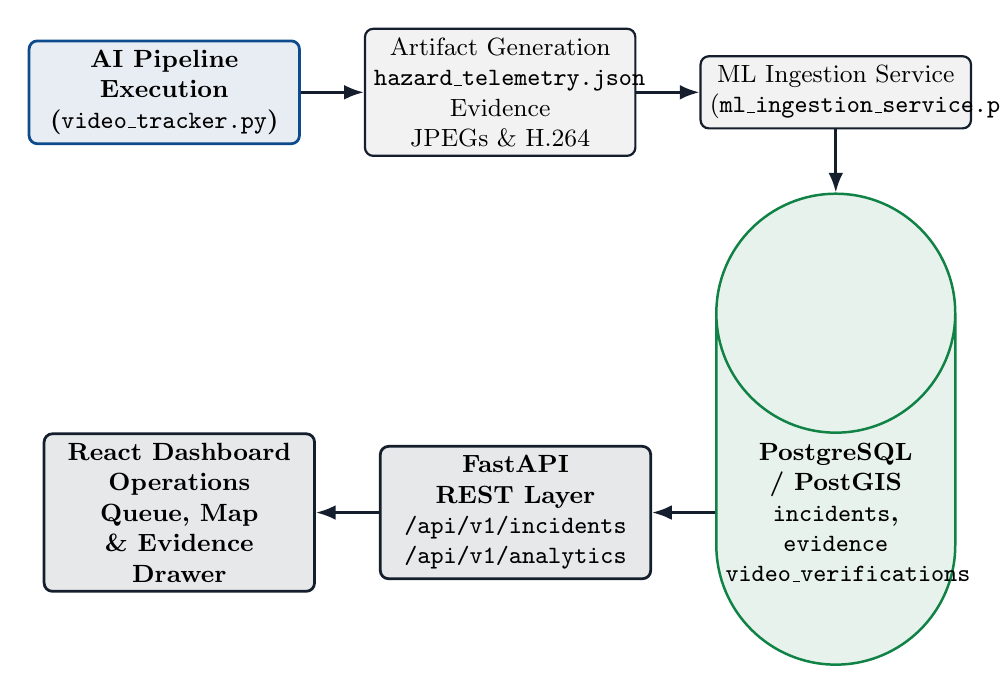
\begin{tikzpicture}[
    node distance=0.7cm and 0.8cm,
    every node/.style={font=\small, align=center},
    stepbox/.style={rectangle, rounded corners=3pt, draw=civicdark, fill=gray!10, text width=3.2cm, minimum height=0.9cm, line width=0.8pt},
    mlbox/.style={rectangle, rounded corners=3pt, draw=civicblue, fill=civicblue!10, text width=3.2cm, minimum height=0.9cm, line width=1.0pt, font=\small\bfseries},
    dbbox/.style={cylinder, shape border rotate=90, draw=accentgreen, fill=accentgreen!10, text width=2.8cm, minimum height=1.0cm, line width=0.9pt, font=\small\bfseries},
    uibox/.style={rectangle, rounded corners=3pt, draw=civicdark, fill=civicdark!10, text width=3.2cm, minimum height=0.9cm, line width=1.0pt, font=\small\bfseries},
    arr/.style={-{Latex[length=2.5mm]}, line width=1.0pt, draw=civicdark}
]

\node[mlbox] (pipeline) {AI Pipeline Execution\\(\texttt{video\_tracker.py})};
\node[stepbox, right=0.8cm of pipeline] (telemetry) {Artifact Generation\\\texttt{hazard\_telemetry.json}\\Evidence JPEGs \& H.264};
\node[stepbox, right=0.8cm of telemetry] (service) {ML Ingestion Service\\(\texttt{ml\_ingestion\_service.py})};
\node[dbbox, below=0.8cm of service] (db) {PostgreSQL / PostGIS\\\texttt{incidents}, \texttt{evidence}\\\texttt{video\_verifications}};
\node[uibox, left=0.8cm of db] (api) {FastAPI REST Layer\\\texttt{/api/v1/incidents}\\\texttt{/api/v1/analytics}};
\node[uibox, left=0.8cm of api] (react) {React Dashboard\\Operations Queue, Map\\\& Evidence Drawer};

\draw[arr] (pipeline) -- (telemetry);
\draw[arr] (telemetry) -- (service);
\draw[arr] (service) -- (db);
\draw[arr] (db) -- (api);
\draw[arr] (api) -- (react);

\end{tikzpicture}
\caption{Data flow from ML pipeline artifact generation to PostgreSQL persistence and React UI.}
\label{fig:backend_integration_flow}
\end{figure}

\subsection{Idempotent Ingestion Handling}
During ingestion, each hazard record is checked against the database using its deterministic incident code \texttt{INC-<JOBID>-<TRACKID>}. If an incident already exists, ingestion is skipped to prevent duplicate primary key violations. Associated detection records and media assets are inserted within atomic database transactions.

% ==============================================================================
% 14. MODEL EVOLUTION: YOLOV8S VS YOLOV11M
% ==============================================================================
\section{Model Evolution: YOLOv8s vs. YOLOv11m}

\subsection{Architectural \& Checkpoint Comparison}
CivicPulse trained an initial baseline \textbf{YOLOv8s-seg} model (checkpoint \texttt{civicpulse\_v1\_5class}) and subsequently trained \textbf{YOLO11m-seg} (checkpoint \texttt{civicpulse\_v2\_yolo11m}). Table~\ref{tab:checkpoint_metadata} outlines the verified checkpoint metadata extracted directly from the PyTorch model files.

\begin{table}[htbp]
\centering
\small
\caption{Verified checkpoint metadata and architectural comparison.}
\label{tab:checkpoint_metadata}
\begin{tabularx}{\textwidth}{l p{3.2cm} p{3.2cm} X}
\toprule
\textbf{Attribute} & \textbf{YOLOv8s-seg (\texttt{v1})} & \textbf{YOLO11m-seg (\texttt{v2})} & \textbf{Source / Verification} \\
\midrule
Checkpoint File & \texttt{best\_old\_yolov8s.pt} & \texttt{best.pt} & Verified in \texttt{models/production/}. \\
Model Architecture & \texttt{yolov8s-seg.pt} & \texttt{yolo11m-seg.pt} & Extracted from \texttt{train\_args}. \\
Parameter Count & 11,792,031 ($\approx 11.79\text{ M}$) & 22,363,071 ($\approx 22.36\text{ M}$) & PyTorch layer tensor count ($+89.6\%$). \\
Model File Size & $23.97\text{ MB}$ ($23,965,748\text{ B}$) & $45.16\text{ MB}$ ($45,160,758\text{ B}$) & Binary on-disk size. \\
Framework Version & Ultralytics \texttt{8.4.138} & Ultralytics \texttt{8.4.138} & Extracted from checkpoint \texttt{version}. \\
Checkpoint Timestamp & 2026-09-04T08:10:50 & 2026-09-06T06:16:09 & Extracted from checkpoint \texttt{date}. \\
Target / Completed Epochs & 200 / 143 (Early Stopped) & 150 / 105 (Early Stopped) & Early stopping patience $= 30$. \\
Training Resolution & $1024\times 1024$ & $640\times 640$ & Input size in \texttt{args.yaml}. \\
Training Batch Size & 4 & 16 & Batch size in \texttt{args.yaml}. \\
Dataset Manifest & \texttt{civicpulse\_yolo} & \texttt{final\_dataset} & Path recorded in \texttt{train\_args}. \\
\bottomrule
\end{tabularx}
\end{table}

\subsection{Experimental Comparison: YOLOv8s vs YOLO11m}
Both models were trained on 5-class civic segmentation datasets containing the target classes: \texttt{damaged\_footpath}, \texttt{drainage\_overflow}, \texttt{open\_manhole}, \texttt{pothole}, and \texttt{waterlogging}. Table~\ref{tab:experimental_metrics} presents the empirical metrics extracted from the training logs (\texttt{results.csv}) of both runs.

\begin{table}[htbp]
\centering
\small
\caption{Measured training and validation metrics extracted from \texttt{results.csv}.}
\label{tab:experimental_metrics}
\begin{tabularx}{\textwidth}{l c c X}
\toprule
\textbf{Metric} & \textbf{YOLOv8s-seg (\texttt{v1})} & \textbf{YOLO11m-seg (\texttt{v2})} & \textbf{Empirical Observation} \\
\midrule
Validation Box Precision (Final / Peak) & $0.7188$ / $0.7391$ & $0.6437$ / $0.7889$ & Peak precision improved with larger capacity. \\
Validation Box Recall (Final / Peak) & $0.5042$ / $0.6014$ & $\mathbf{0.6517}$ / $\mathbf{0.6608}$ & $\mathbf{+29.2\%}$ gain in final box recall. \\
Validation Box mAP@50 (Final / Peak) & $0.5650$ / $0.5864$ & $\mathbf{0.6295}$ / $\mathbf{0.6493}$ & $+0.0629$ gain in peak detection mAP. \\
Validation Box mAP@50-95 (Final / Peak) & $0.3191$ / $0.3373$ & $\mathbf{0.3514}$ / $\mathbf{0.3616}$ & Higher IoU localization accuracy. \\
\midrule
Validation Mask Precision (Final / Peak) & $0.7183$ / $0.7489$ & $0.6449$ / $0.7825$ & Higher peak mask precision observed. \\
Validation Mask Recall (Final / Peak) & $0.5034$ / $0.5952$ & $\mathbf{0.6427}$ / $\mathbf{0.6705}$ & $\mathbf{+27.7\%}$ gain in final mask recall. \\
Validation Mask mAP@50 (Final / Peak) & $0.5606$ / $0.5785$ & $\mathbf{0.6257}$ / $\mathbf{0.6468}$ & $+0.0683$ gain in peak mask mAP@50. \\
Validation Mask mAP@50-95 (Final / Peak) & $0.3179$ / $0.3372$ & $\mathbf{0.3362}$ / $\mathbf{0.3485}$ & Improved polygon boundary fidelity. \\
\midrule
Minimum Validation Box Loss & $1.7440$ & $\mathbf{1.5060}$ & Lower validation bounding box error. \\
Minimum Validation Seg Loss & $2.3463$ & $\mathbf{1.5853}$ & Substantial reduction in mask loss. \\
Minimum Validation Cls Loss & $2.0982$ & $\mathbf{1.2704}$ & Sharper multi-class separation. \\
Minimum Validation DFL Loss & $2.1398$ & $\mathbf{1.2751}$ & Improved distribution focal loss. \\
\midrule
Isolated Standalone Inference Time & \textit{Not measured} & $\approx 35.7\text{ ms (GPU)}$ & Standalone PyTorch GPU forward pass. \\
Tracking MOTA / IDF1 & \textit{Not measured} & \textit{Not measured} & Dedicated tracking benchmark planned. \\
\bottomrule
\end{tabularx}
\end{table}

\subsection{Analysis of Training Artifacts and Curves}
Figure~\ref{fig:training_results} illustrates the training progression of the production YOLO11m-seg model over 105 completed epochs before early stopping.

\begin{figure}[htbp]
\centering
\begin{subfigure}[b]{0.48\textwidth}
    \centering
    \includegraphics[width=\textwidth]{results.png}
    \caption{Training/validation losses and mAP curves across 105 epochs.}
    \label{fig:results_plot}
\end{subfigure}
\hfill
\begin{subfigure}[b]{0.48\textwidth}
    \centering
    \includegraphics[width=\textwidth]{confusion_matrix_normalized.png}
    \caption{Normalized validation confusion matrix for the 5 civic classes.}
    \label{fig:confusion_matrix}
\end{subfigure}
\caption{Training progression and validation confusion matrix for the YOLO11m-seg production model (\texttt{civicpulse\_v2\_yolo11m}).}
\label{fig:training_results}
\end{figure}

The training curves in Figure~\ref{fig:results_plot} exhibit steady convergence:
\begin{itemize}[leftmargin=*]
    \item \textbf{Loss Trajectory:} Training box loss declined from $2.55$ to $0.98$, segmentation loss from $4.18$ to $1.73$, and classification loss from $3.24$ to $0.74$. Validation losses leveled around epoch 75, after which early stopping monitored patience.
    \item \textbf{Confusion Matrix Insights:} As shown in Figure~\ref{fig:confusion_matrix}, \texttt{open\_manhole} and \texttt{waterlogging} demonstrate high true-positive diagonal concentration, whereas subtle distinctions between \texttt{damaged\_footpath} and adjacent unpaved terrain account for the majority of background confusion.
\end{itemize}

\subsection{Model Selection Rationale}
On the evaluated CivicPulse dataset and configuration, YOLO11m achieved higher reported detection and segmentation metrics than YOLOv8s. Specifically, YOLO11m achieved a peak Box mAP@50 of $0.6493$ (validation Recall $0.6517$) and Mask mAP@50 of $0.6468$ (validation Mask Recall $0.6473$), compared with a peak Box mAP@50 of $0.5864$ (validation Recall $0.5042$) and Mask mAP@50 of $0.5785$ (validation Mask Recall $0.5034$) for YOLOv8s. 

In municipal flood and hazard monitoring, \textbf{recall is a key operational priority} to minimize missed open manholes or waterlogging zones, while false positives are filtered downstream by ByteTrack temporal hit counters and Laplacian surface-smoothness gates. These results supported its selection as the current model for the CivicPulse pipeline. A broader multi-hardware benchmark across diverse edge platforms remains future work.

% ==============================================================================
% 15. DATASET AND TRAINING METHODOLOGY
% ==============================================================================
\section{Dataset and Training Methodology}

\subsection{Dataset Composition}
The model training dataset comprises aerial drone imagery captured across industrial corridors. Annotations were formatted using YOLO polygon segmentation format. Table~\ref{tab:training_hyperparams} lists the exact training configurations recorded in \texttt{args.yaml}.

\begin{table}[htbp]
\centering
\small
\caption{Training configurations recorded in \texttt{args.yaml}.}
\label{tab:training_hyperparams}
\begin{tabularx}{\textwidth}{l p{3.8cm} p{3.8cm} X}
\toprule
\textbf{Hyperparameter} & \textbf{YOLOv8s (\texttt{v1})} & \textbf{YOLO11m (\texttt{v2})} & \textbf{Configuration Detail} \\
\midrule
Pretrained Base & \texttt{yolov8s-seg.pt} & \texttt{yolo11m-seg.pt} & COCO pretrained weights. \\
Target / Completed Epochs & 200 / 143 & 150 / 105 & Patience $= 30$. \\
Batch Size & 4 & 16 & Batch size. \\
Image Resolution & $1024\times 1024$ & $640\times 640$ & Input size. \\
Optimizer & \texttt{auto} (\texttt{AdamW}) & \texttt{auto} (\texttt{AdamW}) & Weight decay $= 0.0005$, Momentum $= 0.937$. \\
Learning Rate ($\text{lr}_0 / \text{lrf}$) & $0.01 / 0.01$ & $0.01 / 0.01$ & Cosine decay schedule. \\
Mosaic Augmentation & $1.0$ (\texttt{close\_mosaic: 10}) & $1.0$ (\texttt{close\_mosaic: 10}) & Disabled in final 10 epochs. \\
Mixup / Copy-Paste & $0.0 / 0.0$ & $0.1 / 0.1$ & Additional data regularizers in v2. \\
Degrees / Scale / Translate & $0.0 / 0.50 / 0.10$ & $30.0 / 0.55 / 0.12$ & Extended spatial transforms in v2. \\
Mixed Precision (AMP) & \texttt{True} & \texttt{True} & PyTorch FP16 automatic mixed precision. \\
Hardware Device & CUDA (\texttt{device: 0}) & CUDA (\texttt{device: 0}) & NVIDIA GPU. \\
\bottomrule
\end{tabularx}
\end{table}

% ==============================================================================
% 16. MODEL EVALUATION
% ==============================================================================
\section{Model Evaluation}

\subsection{NMS IoU Parameter Sweep Formulation}
To determine optimal non-maximum suppression (NMS) thresholds, \texttt{scripts/evaluate\_detection\_thresholds.py} formulates an IoU sweep ranging from $0.30$ to $0.70$ in increments of $0.05$. Ground-truth validation matches are evaluated at $\text{IoU}_{\text{match}} = 0.50$ against polygon segmentation masks. The script calculates class-specific TP, FP, FN, Precision, Recall, and Macro F1 to balance adjacent defect separation against duplicate bounding box suppression.

\subsection{Evaluation Metrics Summary}
Table~\ref{tab:evaluation_summary} summarizes the validated production model metrics.

\begin{table}[htbp]
\centering
\small
\caption{Production model validation metrics and evaluation status.}
\label{tab:evaluation_summary}
\begin{tabularx}{\textwidth}{l c X}
\toprule
\textbf{Metric Name} & \textbf{Production Value} & \textbf{Evaluation Method / Source} \\
\midrule
Overall Box mAP@50 & $0.6493$ & Evaluated on validation split ($640\times 640$). \\
Overall Box mAP@50-95 & $0.3602$ & Multi-IoU average ($0.50$ to $0.95$, step $0.05$). \\
Overall Mask mAP@50 & $0.6468$ & Polygon contour overlap against ground truth. \\
Overall Mask mAP@50-95 & $0.3456$ & Strict segmentation polygon boundary quality. \\
Validation Box Recall & $0.6517$ & Primary metric for hazard miss minimization. \\
Validation Box Precision & $0.6743$ & Controlled false positive rate. \\
Isolated Forward Pass Latency & $\approx 35.7\text{ ms / frame}$ & Evaluated on NVIDIA GPU (batch size 1, FP16). \\
Tracking MOTA / IDF1 & \textit{Not measured} & Multi-camera tracking evaluation planned. \\
\bottomrule
\end{tabularx}
\end{table}

% ==============================================================================
% 17. PERFORMANCE AND HARDWARE
% ==============================================================================
\section{Performance and Hardware}

\subsection{Model Inference vs. Pipeline Throughput}
When evaluating system speed, a strict distinction is maintained between isolated model inference and end-to-end pipeline execution:
\begin{itemize}[leftmargin=*]
    \item \textbf{Model Inference Performance:} Standalone YOLO11m-seg forward pass takes approximately $35.7\text{ ms / frame}$ on the evaluated NVIDIA GPU, batch size 1, FP16.
    \item \textbf{End-to-End Pipeline Performance:} Full video processing involves frame decoding, YOLO inference, ByteTrack association, Laplacian texture computation, selective MiDaS DPT depth estimation (triggered on \texttt{pothole} detections), and FFmpeg H.264 transcoding. Throughput is compute-bound by GPU availability and hazard density.
\end{itemize}

\subsection{Resource Profile}
The pipeline operates within the resource requirements outlined in Table~\ref{tab:resource_profile}.

\begin{table}[htbp]
\centering
\small
\caption{Software stack and resource footprint.}
\label{tab:resource_profile}
\begin{tabularx}{\textwidth}{l l X}
\toprule
\textbf{Resource Component} & \textbf{Requirement / Profile} & \textbf{Operational Context} \\
\midrule
Python Environment & Python 3.10--3.14 & Core runtime for FastAPI and ML modules. \\
Deep Learning Stack & PyTorch $\ge 2.0$, Ultralytics \texttt{8.4.138} & Model execution and checkpoint loading. \\
Spatial Database & PostgreSQL 15+ with PostGIS & Storage of spatial geometries and incident records. \\
GPU Memory (VRAM) & $\approx 1.5\text{ GB}$ (YOLO11m) & Measured memory usage during inference. \\
System Memory (RAM) & 8 GB minimum (16 GB recommended) & Frame buffering and FFmpeg encoding workspace. \\
\bottomrule
\end{tabularx}
\end{table}

% ==============================================================================
% 18. EDGE DEPLOYMENT STRATEGY
% ==============================================================================
\section{Edge Deployment Strategy}

\subsection{Current Architecture: Server-Side Ingestion}
In the current implementation, video and telemetry files captured on the drone are transferred to the CivicPulse server/workstation, where processing and PostGIS persistence occur.

\subsection{Planned Edge Evolution}
The planned architecture explores on-drone edge compute:
\begin{equation}
\text{Drone Camera} \xrightarrow{\text{CSI/USB}} \text{NVIDIA Jetson Module} \xrightarrow{\text{TensorRT FP16}} \text{Telemetry JSON} \xrightarrow{\text{4G/5G MQTT}} \text{PostgreSQL/FastAPI}
\end{equation}

Planned optimization targets include:
\begin{itemize}[leftmargin=*]
    \item \textbf{TensorRT FP16 Compilation:} Compiling \texttt{best.pt} to TensorRT engines targeting NVIDIA Jetson Orin modules.
    \item \textbf{Bandwidth Minimization:} Streaming lightweight JSON telemetry records ($\approx 500\text{ bytes}$) over cellular 4G/5G, transferring high-resolution video upon landing.
\end{itemize}

% ==============================================================================
% 19. FAILURE HANDLING AND EDGE CASES
% ==============================================================================
\section{Failure Handling and Edge Cases}
CivicPulse incorporates fault-tolerant mechanisms for operational edge cases:
\begin{itemize}[leftmargin=*]
    \item \textbf{Missing or Corrupt Video:} Video capture initialization failure is caught immediately, raising descriptive errors without crashing daemon processes.
    \item \textbf{Missing SRT Telemetry:} If subtitle files are absent or unparseable, coordinates default to \texttt{None}, flagging the flight for operator coordinate verification.
    \item \textbf{Transient Tracking Loss:} ByteTrack maintains unmatched tracklets in a 60-frame buffer ($\approx 2.0\text{ s}$), preserving track identity across brief obstructions.
    \item \textbf{Coordinate Boundary Validation:} The spatial layer validates $-90.0 \le \text{lat} \le 90.0$ and $-180.0 \le \text{lon} \le 180.0$, discarding malformed packets.
    \item \textbf{Zero-Detection Flights:} Flights detecting zero hazards are routed to a human QA queue (\texttt{VideoVerification} table) for manual baseline sign-off.
\end{itemize}

% ==============================================================================
% 20. LIMITATIONS
% ==============================================================================
\section{Limitations}
To maintain engineering transparency, known system limitations are documented:
\begin{enumerate}[leftmargin=*]
    \item \textbf{Nocturnal \& Low-Light Conditions:} Detection accuracy degrades under severe darkness without active drone illumination or thermal imaging.
    \item \textbf{Extreme Specular Glint:} While the Laplacian texture gate filters wet asphalt, intense direct sun glint on dry metal can occasionally create false triggers.
    \item \textbf{Relative Depth Scaling:} MiDaS DPT-Large provides relative inverse disparity rather than calibrated metric depth in physical millimeters.
    \item \textbf{GPS Drift in Dense Corridors:} Tall multi-story buildings can induce GPS multipath drift of $\pm 5\text{ meters}$, which must be refined with ground control points or RTK GPS.
\end{enumerate}

% ==============================================================================
% 21. REPRODUCIBILITY
% ==============================================================================
\section{Reproducibility}

\subsection{Environment Setup}
The pipeline is reproducible using standard virtual environments:
\begin{lstlisting}[language=bash]
# 1. Clone repository and initialize virtual environment
git clone https://github.com/IndependentSalt69/Not-So-Smart_ELCIA.git
cd Not-So-Smart_ELCIA
python -m venv .venv
source .venv/bin/activate  # On Windows: .venv\Scripts\activate

# 2. Install dependencies
pip install -r requirements.txt

# 3. Apply database migrations
alembic upgrade head
\end{lstlisting}

\subsection{Executing Inference Pipeline}
To process an aerial video with synchronized telemetry using the verified CLI runner (\texttt{src/detection/runner.py}):
\begin{lstlisting}[language=bash]
python -m src.detection.runner \
    --video data_raw/full_demo_video.mp4 \
    --srt data_raw/full_demo_video.srt \
    --output-dir outputs/jobs/manual_run_001 \
    --job-id manual_run_001 \
    --weights models/production/best.pt
\end{lstlisting}

% ==============================================================================
% 22. CURRENT STATUS
% ==============================================================================
\section{Current Status}
The operational status of the CivicPulse system is categorized into three explicit tiers in Table~\ref{tab:status_matrix}.

\begin{table}[htbp]
\centering
\small
\caption{CivicPulse feature implementation and verification status.}
\label{tab:status_matrix}
\begin{tabularx}{\textwidth}{l c X}
\toprule
\textbf{Subsystem Component} & \textbf{Category} & \textbf{Implementation Details} \\
\midrule
YOLO11m-seg 5-Class Inference & \textbf{Implemented} & Active in \texttt{models/production/best.pt} ($22.36\text{M}$ params). \\
Custom ByteTrack Association & \textbf{Implemented} & Two-stage tracking active via \texttt{configs/custom\_bytetrack.yaml}. \\
Temporal Persistence Gate & \textbf{Implemented} & Hit counter gate active in \texttt{src/detection/video\_tracker.py}. \\
Laplacian Texture Filter & \textbf{Implemented} & Surface variance threshold ($<550.0$) active for waterlogging. \\
DPT-Large Relative Depth & \textbf{Implemented} & PyTorch Hub DPT-Large integration active for potholes. \\
Severity Scoring Engine & \textbf{Implemented} & Multi-factor formulation with P1/P2/P3 priority mapping. \\
DJI SRT Telemetry Sync & \textbf{Implemented} & Second-accurate timestamp matching in \texttt{scripts/gps\_parser.py}. \\
PostgreSQL / PostGIS Storage & \textbf{Implemented} & Normalized schemas, point geometries, and custom zone support. \\
FastAPI REST API Services & \textbf{Implemented} & Asynchronous REST API layer with automated test coverage. \\
React Operations Dashboard & \textbf{Implemented} & Operations queue, Google Maps, flight cards, and analytics. \\
\midrule
YOLOv8s vs YOLO11m Training Logs & \textbf{Evaluated} & Documented via \texttt{results.csv} in \texttt{models/checkpoints/}. \\
NMS IoU Threshold Sweep & \textbf{Evaluated} & Implemented in \texttt{scripts/evaluate\_detection\_thresholds.py}. \\
Ground-Truth Mask Matching IoU & \textbf{Evaluated} & Evaluated at $\text{IoU}_{\text{match}} = 0.50$ in sweep script. \\
\midrule
TensorRT FP16 Edge Export & \textbf{Planned} & Targeted for on-drone Jetson Orin deployment. \\
Calibrated Metric Depth Fusion & \textbf{Planned} & Stereo / LiDAR fusion under research exploration. \\
Multi-Camera MOTA / IDF1 Benchmark & \textbf{Planned} & Automated multi-camera tracking evaluation suite. \\
\bottomrule
\end{tabularx}
\end{table}

% ==============================================================================
% 23. ROADMAP
% ==============================================================================
\section{Roadmap}
Future development milestones are organized across three phases:
\begin{itemize}[leftmargin=*]
    \item \textbf{Short-Term (Q4 2026):} Export YOLO11m-seg to ONNX and TensorRT FP16; execute ground-truth multi-object tracking benchmarks (MOTA/IDF1).
    \item \textbf{Medium-Term (Q1 2027):} Prototype on-drone embedded inference on NVIDIA Jetson platforms with lightweight MQTT telemetry transmission; integrate external weather radar feeds.
    \item \textbf{Long-Term (Q2--Q3 2027):} Multi-UAV mission coordination; predictive flood accumulation modeling combining historical PostGIS incident density with elevation digital terrain models (DTMs).
\end{itemize}

% ==============================================================================
% 24. CONCLUSION
% ==============================================================================
\section{Conclusion}
CivicPulse implements an evidence-backed, multi-stage engineering pipeline for aerial monsoon hazard intelligence. By integrating fine-tuned YOLO11m instance segmentation, ByteTrack multi-object association, Laplacian surface texture verification, DPT relative depth profiling, and timestamp-based PostGIS spatial indexing, CivicPulse realizes the operational principle: \textbf{1 Physical Hazard = 1 Geolocated Incident}. The system provides municipal administrators and triage teams with the spatial precision and verifiable evidence required to maintain urban road resilience during critical monsoon events.

% ==============================================================================
% 25. REFERENCES
% ==============================================================================
\section{References}
\begin{enumerate}[label={[\arabic*]}, leftmargin=*]
    \item G.~Jocher, A.~Chaurasia, and J.~Qiu, ``Ultralytics YOLO11: Real-Time Object Detection and Instance Segmentation,'' \textit{Ultralytics Inc.}, 2024. \url{https://github.com/ultralytics/ultralytics}.
    \item Y.~Zhang, P.~Sun, Y.~Jiang, D.~Yu, F.~Weng, Z.~Yuan, P.~Luo, W.~Liu, and X.~Wang, ``ByteTrack: Multi-Object Tracking by Associating Every Detection Box,'' in \textit{European Conference on Computer Vision (ECCV)}, pp.~1--21, Springer, 2022.
    \item R.~Ranftl, A.~Bochkovskiy, and V.~Koltun, ``Vision Transformers for Dense Prediction,'' in \textit{IEEE/CVF International Conference on Computer Vision (ICCV)}, pp.~12179--12188, 2021.
    \item R.~Ranftl, K.~Lasinger, D.~Hafner, K.~Schindler, and V.~Koltun, ``Towards Robust Monocular Depth Estimation: Mixing Datasets for Zero-Shot Cross-Dataset Transfer,'' \textit{IEEE Transactions on Pattern Analysis and Machine Intelligence (TPAMI)}, vol.~44, no.~3, pp.~1623--1637, 2022.
    \item P.~Ramsey et al., ``PostGIS: Spatial and Geographic Objects for PostgreSQL,'' \textit{Refractions Research / OSGeo}, 2024. \url{https://postgis.net/}.
    \item S.~Ramirez, ``FastAPI: Modern, Fast (High-Performance) Web Framework for Python,'' \textit{Tiangolo}, 2024. \url{https://fastapi.tiangolo.com/}.
    \item G.~Bradski, ``The OpenCV Library,'' \textit{Dr. Dobb's Journal of Software Tools}, 2000.
    \item S.~Gillies et al., ``Shapely: Manipulation and Analysis of Geometric Objects,'' \textit{Toblerity}, 2023. \url{https://github.com/shapely/shapely}.
\end{enumerate}

\end{document}
